\documentclass[../main.tex]{subfiles}
\graphicspath{{\subfix{../images/}}}
\begin{document}

\chapter{Results and Discussion}
\section{Conclusion}

The purpose of this project was to develop a puzzle video game to teach students about electric circuits. The game was designed to be engaging and challenging, and it incorporated a variety of gamification elements, such as rewards, leaderboards, and achievements.

Due to limited budget and time, only 75\% of the originally planned features were implemented. However, we are still working on adding the rest of the features. We will also be conducting testing to ensure that the game is both educational and fun.

Once the game is complete, we will follow up with the students who filled out the original survey and said they would be interested in trying the game. We will then publish a separate results paper that will discuss the findings of our study.

We believe that this game has the potential to be a valuable tool for teaching students about electric circuits. We are excited to continue working on the game and to share it with students in the future.

\section{Challenges}

One of the biggest challenges that we faced was learning about electric circuits in order to make sure that our simulation was accurate. We had to learn about the different components of circuits, how they work together, and how to simulate them in our game.

Another challenge that we faced was designing and implementing the system in C\# using various design patterns. We needed to implement a lot of features, such as undo, move, flip, copy, paste, electronic terminal connections, VFX and SFX, animations, lighting, and so much more.

\section{Lessons Learned}

We learned a lot from this project. We learned about clean coding principles, agile (Scrum) project management, teamwork between engineers, programmers, artists, and game designers, and various algorithms like linear interpolation for animation, and graphs for electric circuits connections.

\section{Plans for the Future}

We have a lot of plans for the future of this project. We plan to add more components to the game, such as capacitors, inductors, transistors, and various ICs. We also plan to add minigames to aid certain skills, such as reading resistor values and datasheets. We also plan to add a textbook in the game (in-game encyclopedia).

Once the game is complete, we will conduct public testing. After that, we will polish the game, market it, and publish it on Steam.

We are excited to continue working on this project and to share it with students in the future. We believe that this game has the potential to be a valuable tool for teaching students about electric circuits.

\newpage
\section{Screenshots from the game}
\begin{figure}[!ht]
    \centering
    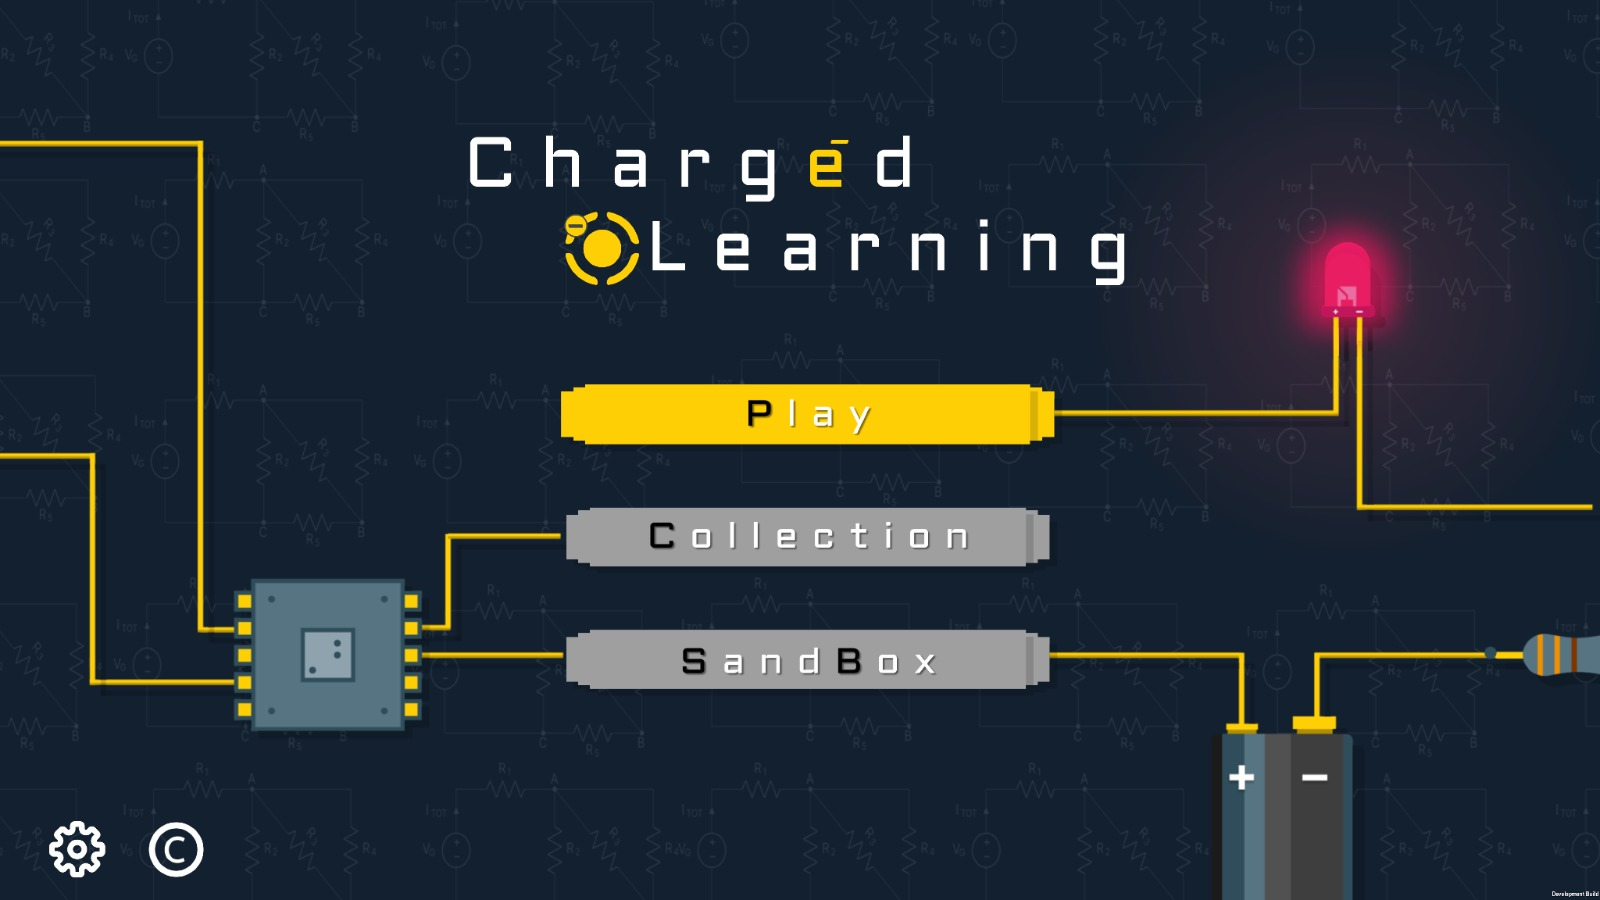
\includegraphics[scale=0.3]{images/chapter5/main_menu.jpeg}
    \caption{Main menu}
    \label{main_menu}
\end{figure}

\begin{figure}[!ht]
    \centering
    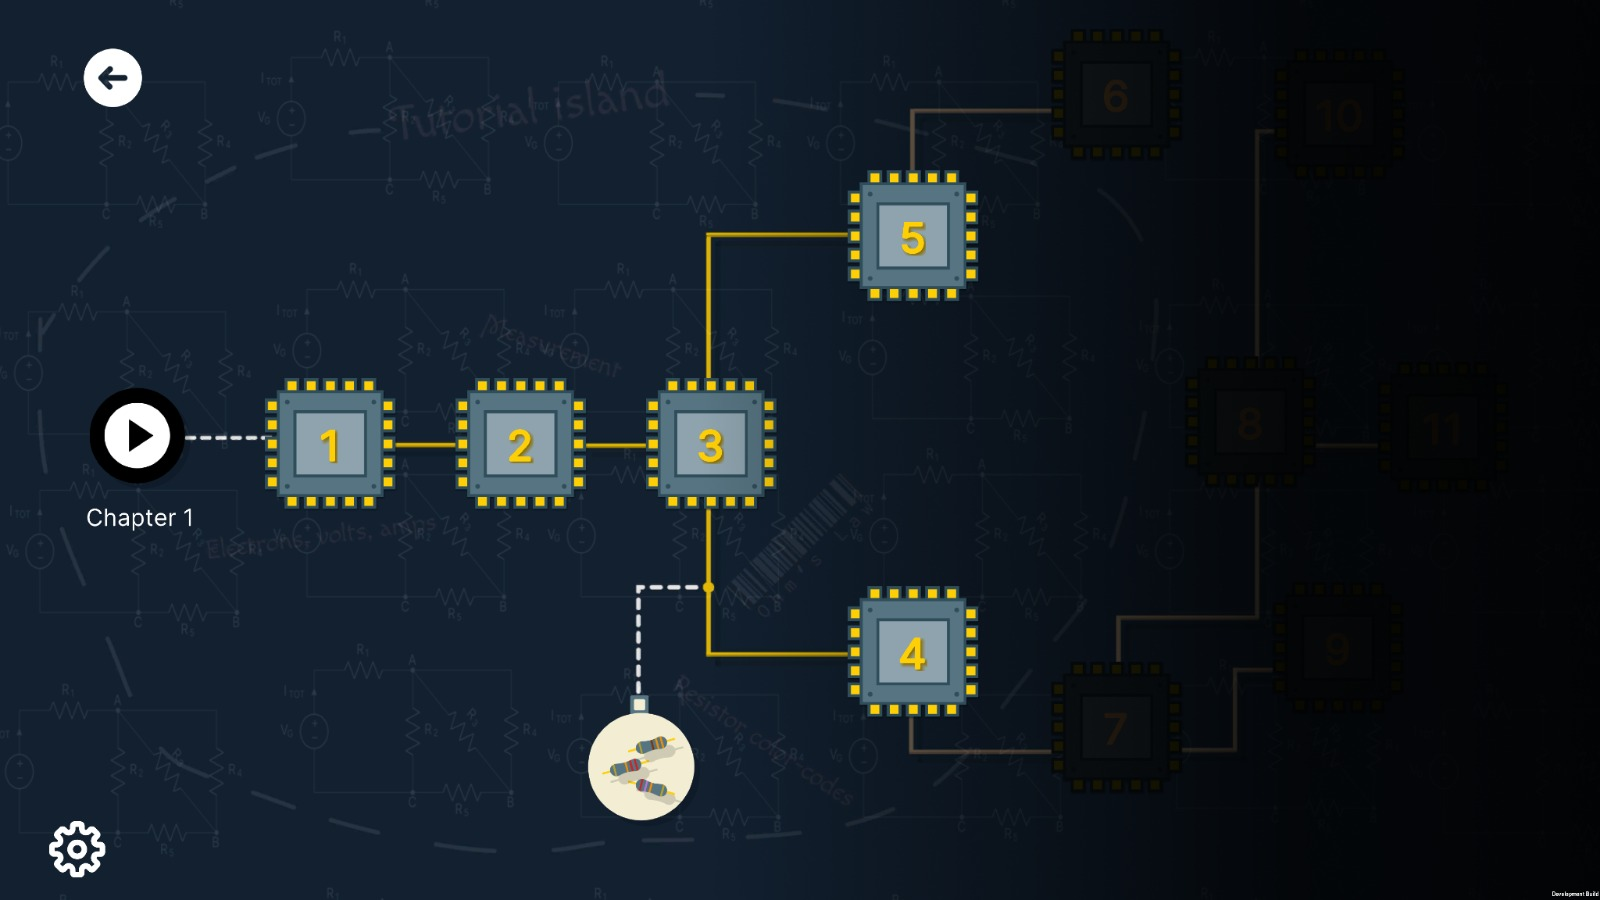
\includegraphics[scale=0.3]{images/chapter5/level_tree.jpeg}
    \caption{Level tree}
    \label{level_tree}
\end{figure}

\begin{figure}[!ht]
    \centering
    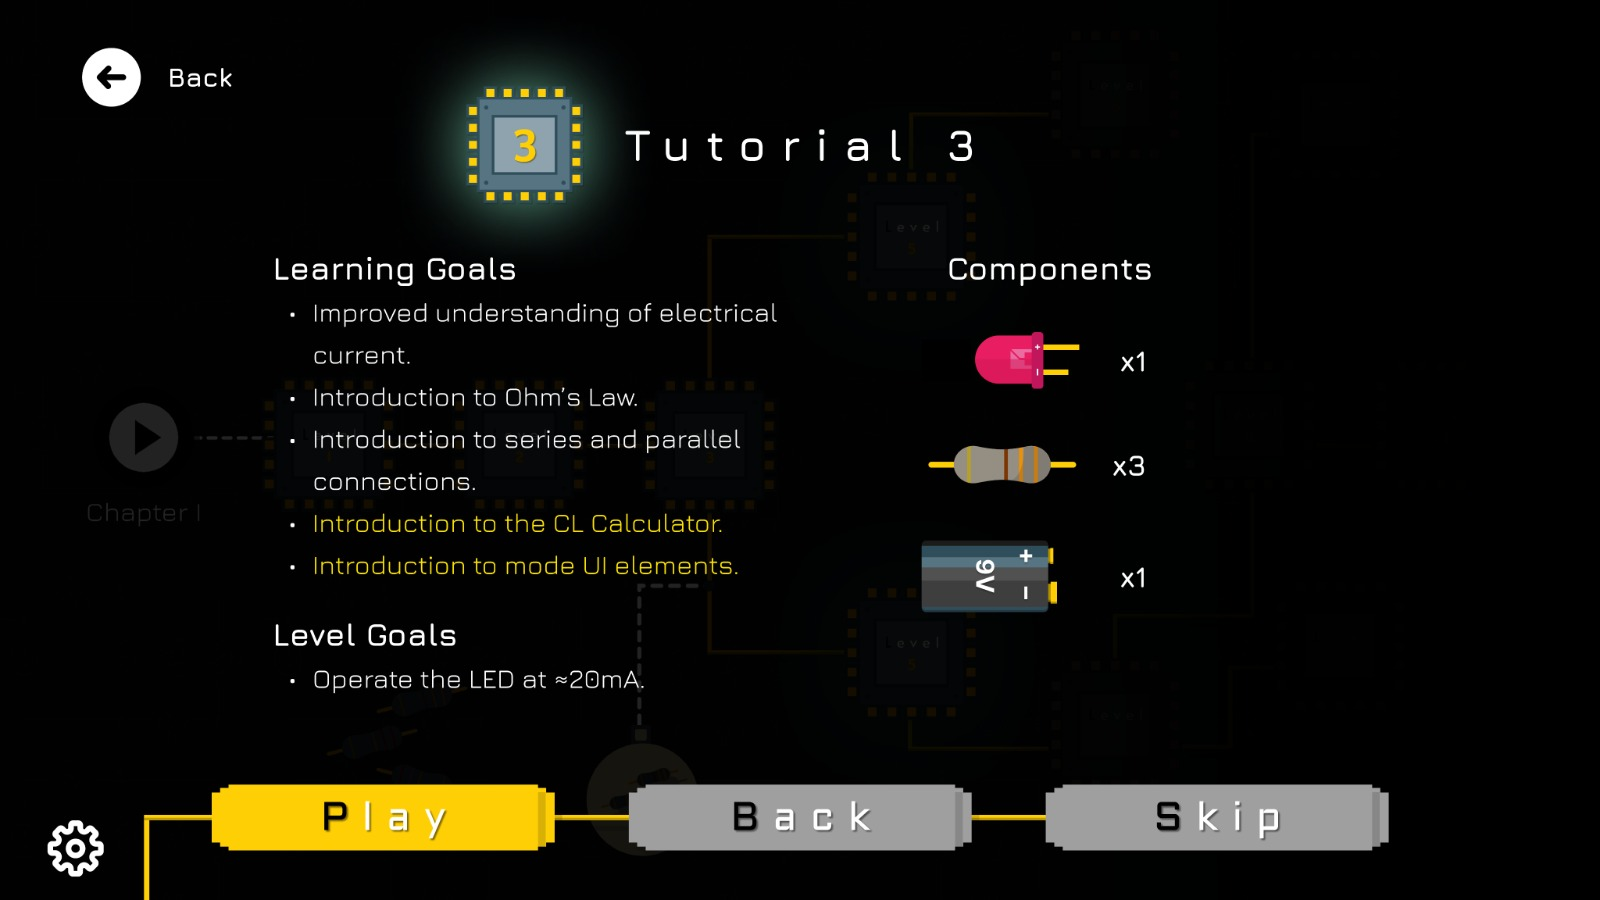
\includegraphics[scale=0.3]{images/chapter5/level_overview.jpeg}
    \caption{Level overview}
    \label{level_overview}
\end{figure}

\begin{figure}[!ht]
    \centering
    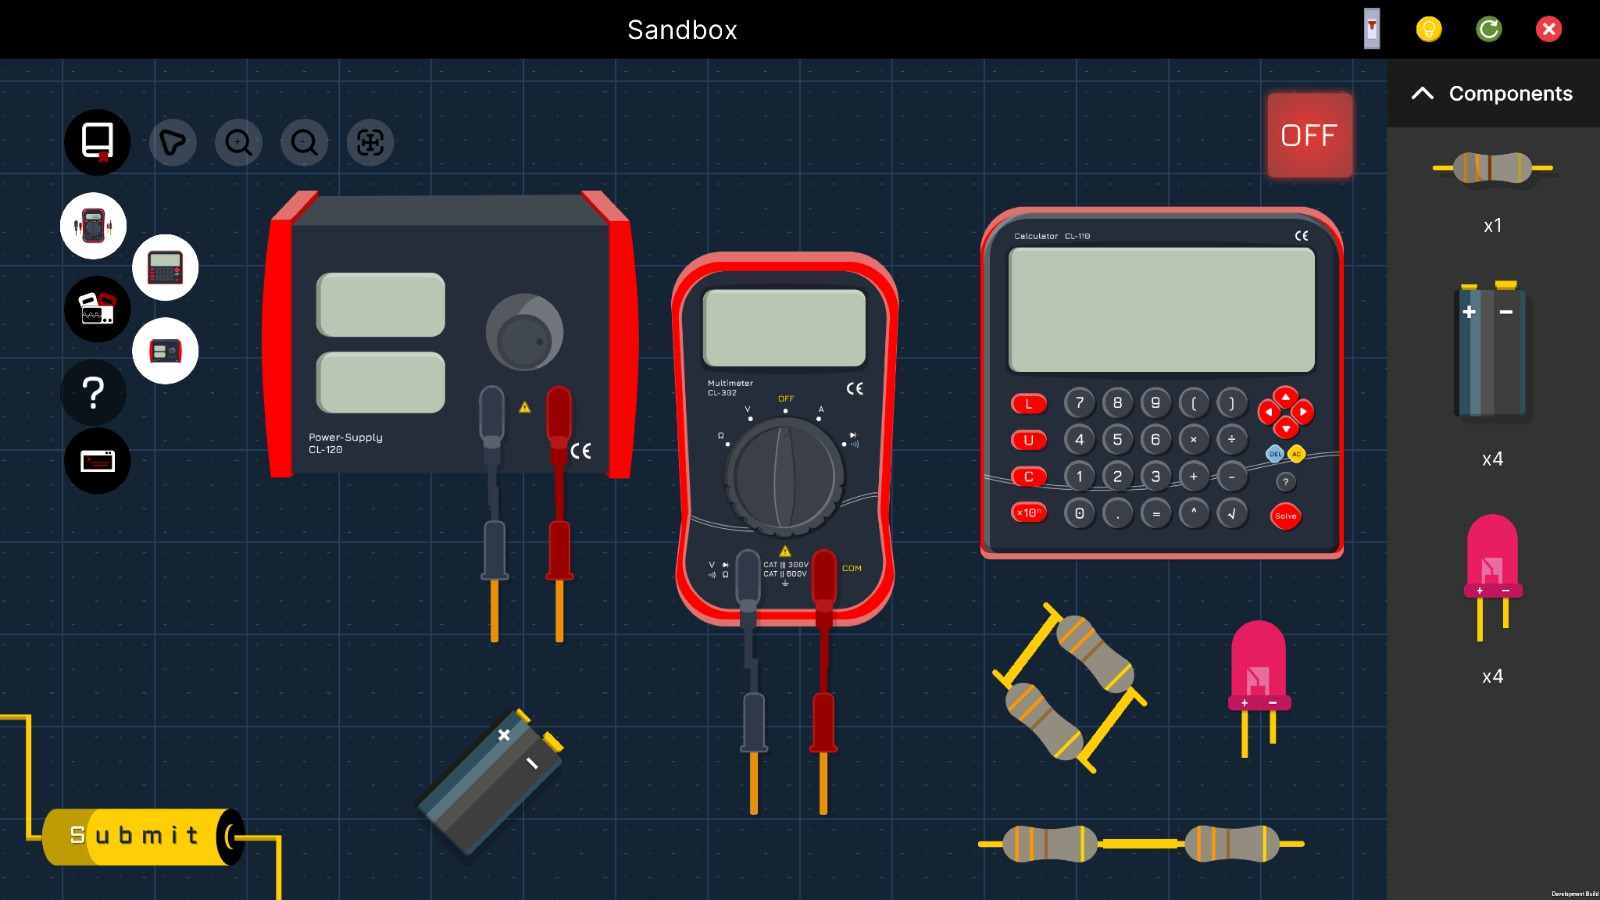
\includegraphics[scale=0.3]{images/chapter5/sandbox.jpeg}
    \caption{Sandbox mode}
    \label{sandbox}
\end{figure}

\begin{figure}[!ht]
    \centering
    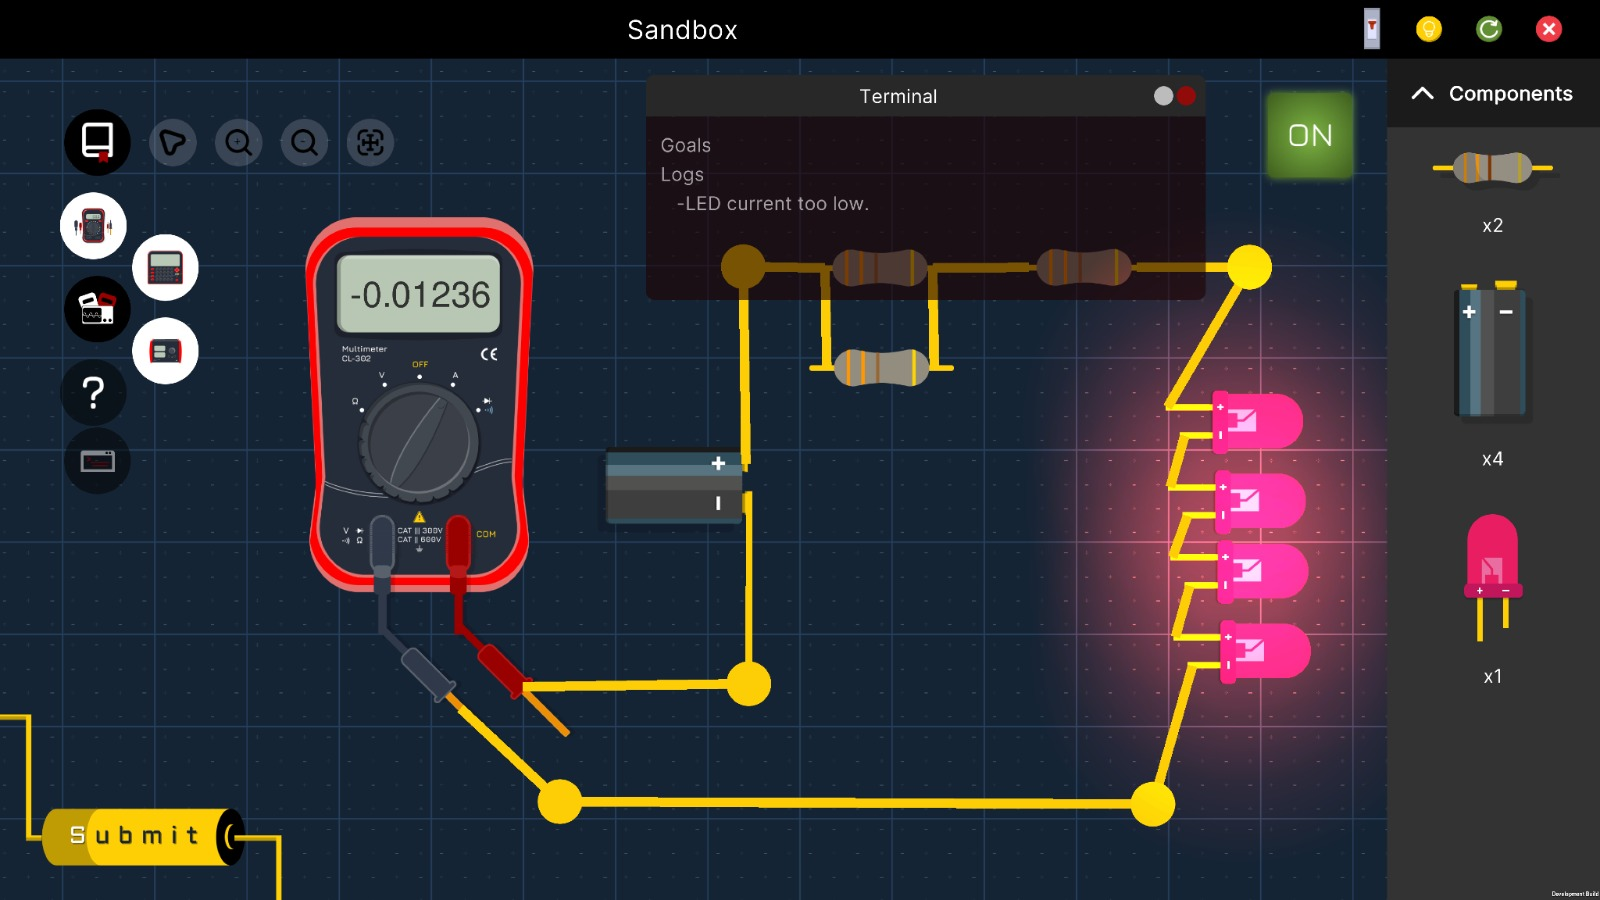
\includegraphics[scale=0.3]{images/chapter5/led_array.jpeg}
    \caption{LED array}
    \label{led_array}
\end{figure}    
\end{document}
